\documentclass[output=paper,colorlinks,citecolor=brown
% ,hidelinks
% showindex
]{langscibook}
\author{Levente Alekszejenkó\orcid{0000-0002-3196-1950}\affiliation{Deparment of Measurement and Information Systems, Budapest University of Technology and Economics}
        }
\title{Explanations based on Training Datasets}
\abstract{}

%move the following commands to the "local..." files of the master project when integrating this chapter
\usepackage{tabularx}
\usepackage{langsci-optional}
\usepackage{langsci-gb4e}
\bibliography{localbibliography}
\usepackage{hyperref}
\newcommand{\orcid}[1]{}

\IfFileExists{../localcommands.tex}{
   \addbibresource{../localbibliography.bib}
   % add all extra packages you need to load to this file  
\usepackage{tabularx} 

% \usepackage{langsci-branding}
\usepackage{langsci-optional}
 

   \newcommand*{\orcid}{}

   \input{../localhyphenation}
   \boolfalse{bookcompile}
   \togglepaper[23]%%chapternumber
}{}

\begin{document}
\maketitle

\section{Introduction}
As Artificial Intelligence (AI) tends to be a part of each modern IT system, explanations of its predictions also gain importance. However, there are multiple white-box, self-explaining models (e.g., decision trees, Bayesian networks); many current AI models are black-box ones. Consequently, we shall provide methods that can effectively yet intelligibly describe these models' predictions. To this end, we will see two relatively simple approaches that can provide explanations of black-box classifiers.

Let us assume that the examined classifier models are trained optimally. By optimal training, we mean that the model neither under nor overfits the training data. Or by another definition, if we select two classifiers trained on the same training data, we cannot distinguish them by their prediction quality. Furthermore, we may assume that each adequately complex model can reach optimality on their training datasets. As a result, if we got two (optimally trained) black-box models (on some datasets), their forecasting capabilities can only differ due to various training data.

Consequently, exploring the characteristics of training datasets can provide explanations for black-box AI predictors. In the continuation, two sample-based explanation methods will be presented.

\section{Subspace of the Training Samples}
\label{sec:space}
Without loss of generality\footnote{We can represent categorical features as e.g. one-hot encoded vectors.}, let us suppose that the training data is numerical. This way, the features can be interpreted as vectors in $\mathbb{R}^d$, where $d$ corresponds to the number of the features.

In a classification problem, the classes usually form a polytope\footnote{If a class corresponds to an unbounded object in $\mathbb{R}^d$, we can consider it bounded by a surface at the lowest/highest number of its computer representation.} in $\mathbb{R}^d$. Therefore, the fundamental goal of a classifier is to find the boundaries of these polytopes. If these boundaries are known, the classification problem is the same as asking whether a particular point is inside a certain polytope (a test sample belongs to a class).

We can also reason that points close to each other (by either L1 or L2-norm) correspond to similar records. Please note that similarity does not necessarily indicate the two samples belong to the same class. E.g., they might be close, yet on another side of the boundary of a class' polytope.

This geometrical reasoning can provide a sound mathematical background for explaining the predictions of an AI classifier based on its training data set. 

\section{ProtoDash}
\label{sec:protodash}
Following the taxonomy of \cite{aix360}, the ProtoDash \cite{protodash} method is a sample-based explanation generator tool that can explain both datasets and models. It generates local explanations in a post-hoc manner providing similar training records to the test record we want to explain. The ProtoDash is a general tool that can handle textual, tabular, and image data.

If the Reader is interested, one can find the exact definition of the ProtoDash algorithm in \cite{protodash}. Moreover, \href{https://aix360.mybluemix.net/}{IBM's AI~Explainability~360}\footnote{Last visited on 29-11-2022.}, along with many other techniques, provides an open-source implementation of the ProtoDash algorithm in Python. Hence, in the following, rather than discussing implementation questions, we will focus on the usage and understanding of the algorithm.

\subsection{ProtoDash to Explain a Prediction}
We can select a particular test sample and feed it into our classifier model. As a result, we will obtain a predicted class for the test sample. Naturally, one might be curious about why the model opts for this class. It would be a well-founded explanation if we could show similar training records to our test sample.

\begin{figure}[h!]
    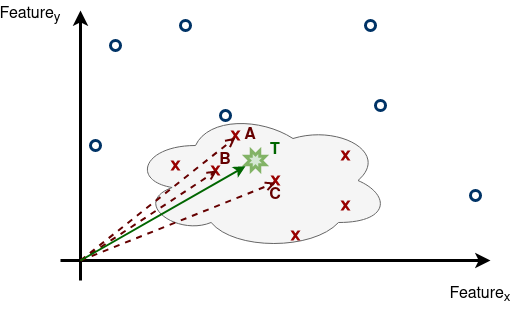
\includegraphics[width=.85\textwidth]{protodash1.png}
    \caption{An example of ProtoDash prediction explanation. Different training sample points are depicted in $\mathbb{R}^2$. The polytope of records having a red cross as a label is depicted by a gray background. We want to explain the $T$ test sample, in other words, we want express the $\mathbf{t}$ vector as convex combination of another vectors. For example, we might obtain that $\mathbf{t} \approx 0.4 \mathbf{a} + 0.2 \mathbf{b} + 0.4 \mathbf{c}$.}
    \label{fig:proto1}
\end{figure}

Translating this to the geometric reasoning of Section~\ref{sec:space}, it would mean that we have to show which training samples approximate the test sample the best. In other words, we want to find a minimal $L$ list of vectors (training samples) of which $\zeta^{(L)}$ convex combination gives (or at least approximates well) the test sample, see Figure~\ref{fig:proto1}.

ProtoDash will return the $(L, \zeta^{(L)})$ pair if its $X^{(1)}$ target set is our test sample, and its $X^{(2)}$ source set parameter is the training dataset. The resulted vector combination is the explanation, as it provides intelligible samples, similar to the test record. 

\subsection{ProtoDash to Explain a Dataset}
Besides explaining a concrete test sample, ProtoDash is also capable of characterizing a whole (training) dataset by providing prototypical records. To this end, we shall set both $X^{(1)}$ and $X^{(2)}$ to be this dataset. Then, the resulted $(L, \zeta^{(L)})$ pair contains the prototype vectors that can describe the dataset.

\begin{figure}[h!]
    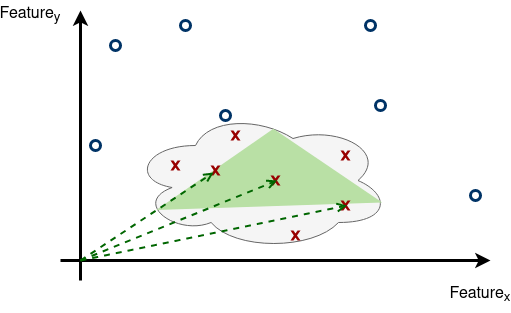
\includegraphics[width=.85\textwidth]{protodash2.png}
    \caption{An example of ProtoDash dataset description. Now, we are interested in what characterizes the red cross labeled samples. To this end, we generate an explanation with ProtoDash. In the first iteration, ProtoDash will select a sample which is closest to the expected value of the dataset. After that, it expands the set of prototypical training records until additional training samples significantly helps to characterize the dataset. Within each step, ProtoDash finds a weighting of the prototypical vectors that is maximal; resulting in a simpler polytope, trying to cover the polytope defined by the training set. In the figure, prototypical samples are marked by green arrows; and their induced maximal polytope is illustrated as the green triangle.}
    \label{fig:proto2}
\end{figure}

Because, in this setup, we want to have a minimal set of vectors that approximates well the whole dataset. In geometrical terms, we want to characterize the polytope induced by the records. Hence, ProtoDash, in this case, will approximate this polytope from the inside with a smaller and simpler polytope as in Figure~\ref{fig:proto2}. The latter is induced by the vectors in $L$ with corresponding weights $\zeta^{(L)}$.

\section{LIME}

ProtoDash, described in Section~\ref{sec:protodash}, has one major drawback, namely, it requires the whole training dataset. However, in most cases, we only got a pre-trained black-box model without having a populous training dataset.

So, given only the classifier model, we want to explain its prediction on a test sample. We can still feed in a variety of similar test inputs and check whether or not they result in identical class prediction to the test sample. In this way, we want to discover where the boundaries of the class' polytope lay in $\mathbb{R}^d$.

The Local Interpretable Model-Agnostic Explanations (LIME) \cite{lime} tool is fundamentally based on the above idea. LIME also has an open-source implementation, accessible from its \href{https://homes.cs.washington.edu/~marcotcr/blog/lime/}{webpage}.\footnote{Last visited on 30-11-2022.} Again, rather than discussing implementation details, we will provide a brief overview of LIME.

LIME, as implied by its name, is model-agnostic, and can be adapted to generate explanations for tabular, textual, and image data.

\subsection{LIME to Explain a Prediction}

\begin{figure}[h!]
    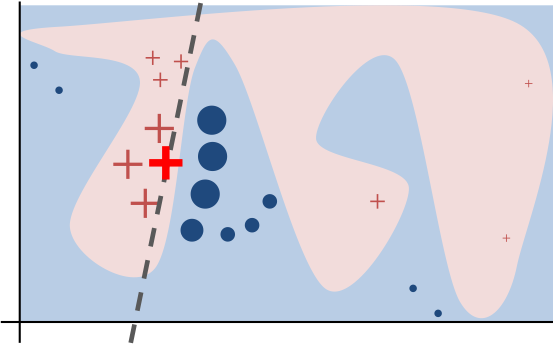
\includegraphics[width=.6\textwidth]{lime.png}
    \caption{An example of LIME. Decision classes are denoted as blue/pink backgrounds. The red cross is the test sample being explained, the other markers correpsond to the perturbated data points, and their sizes reflects their distance from the test sample. The dahsed line is the learned explanation, which is locally (but not globally) faithful. Source: \cite{lime}}
    \label{fig:lime}
\end{figure}

To understand why a classifier predicted a given class for input data, we can use LIME to obtain a local explanation. To this end, LIME generates samples in the locality of our test record by perturbing some of its features. This perturbed set of data will be fed into the model. Based on the class labels of these data (weighted by their distance from the test record in the feature space), LIME approximates the polytope boundary by a simple linear model, see Figure~\ref{fig:lime}. This boundary estimation will provide an intelligible explanation of the class prediction.

\subsection{LIME to Explain a Model}
If we are interested in more than understanding a single prediction, LIME can also help explain a black-box predictor. To do so, we shall feed many test samples into the LIME algorithm to achieve an explanation of the whole classifier model. In other words, we want to approximate the global explanation model by a set of local explanations. In that case, LIME can return an $\mathbf{I}$ vector of the features that effectively outline their importance in the prediction.

\section{Conclusion}
As AI is a rapidly advancing technology, there is a demand to interpret its predictions. However, there are many comprehensible, self-explaining models; many others are too complex to be understood by human beings. To explain the predictions of such black-box models, we can provide some similar training examples to the test data e.g. by the shown ProtoDash algorithms.

Unfortunately, we seldom have access to the complete training data of an already-trained classifier. Then, we might try to interpret the model itself. LIME provides a method that can either explain a concrete prediction or describe the model itself.

\sloppy
\printbibliography[heading=subbibliography,notkeyword=this]
\end{document}
